%!TEX root = ./jctt.tex

The order of accuracy, diffusion limit, and solution convergence were tested in 1D slab geometry with two Eddington factor representations and two scattering term reconstruction methods. The Eddington factor was represented as a piecewise constant with discontinuous jumps at the cell edges and as linear function using the MFEM basis functions. The scattering term reconstruction methods were no reconstruction and maintaining van Leer limited slopes with the MFEM cell centers. The no reconstruction method set the the left and right discontinuous scalar flux to the MFEM edge scalar flux:
	\begin{equation} 
		\phi_{i,L/R} = \phi_{i\mp1/2} \,,
	\end{equation}
where the left hand side is the flux used in the LLDG scattering term and the right hand side the MFEM drift diffusion scalar flux. 
% Maintaining slopes with the MFEM edge values was done according to: 
% 	\begin{equation} \label{eq:edgeReconstruction}
% 		\phi_{i,L/R} = \phi_i \mp \half\left(\phi_{i+1/2} - \phi_{i-1/2}\right) \,.
% 	\end{equation}
The van Leer cell centered reconstruction is: 
	\begin{equation} \label{eq:vanLeer}
		\phi_{i,L/R} = \phi_i \mp \frac{1}{4} \xi_\text{van Leer} \left[ \left(\phi_{i+1} - \phi_{i}\right) + 
			\left(\phi_{i} - \phi_{i-1}\right)\right] \,
	\end{equation}
where $\xi_\text{van Leer}$ is the van Leer slope limiter given in \cite{}. This reconstruction method is especially important for radiative transfer calculations because the MFEM discretized temperature equation will only have cell centered values. 

\subsection{Order of Accuracy}
The Method of Manufactured Solutions (MMS) was used to compare the accuracy of the VEF method as the cell width was decreased. The L2 norm of the difference between the numerical and MMS solution was compared at five logarithmically spaced cell widths between \SI{0.5}{mm} and \SI{0.01}{mm}. A line of best fit of the form 
	\begin{equation} 
		E = C h^n 
	\end{equation}
was used to find the order of accuracy, $n$, and the constant of proportionality, $C$, of the numerical error, $E$. These values along with the coefficient of correlation are provided in Table \ref{tab:mms} for all six permutations of the two Eddington representation methods and three slope reconstruction methods. All of the permutations are second order accurate and have similar overall accuracy. This suggests that Eddington representation and slope reconstruction do not affect numerical accuracy. It is also a testament to the robustness of the VEF method as the inconsistent, partially consistent, and fully consistent variations all performed similarly. 
	\begin{table}[!h] \centering
	\begin{tabular}{|c|c|c|c|c|}
	\hline
	\hline
	Reconstruction Method & Edd. Representation & Order & $C$ & $R^2$ \\ 
	\hline
		None & Constant & \num{1.997} & \num{0.682} & \num{9.9999e-01} \\
None & Linear & \num{1.998} & \num{0.687} & \num{1.0000e+00} \\
Center & Constant & \num{2.007} & \num{0.726} & \num{9.9992e-01} \\
Center & Linear & \num{2.009} & \num{0.732} & \num{9.9991e-01} \\

	\hline
	\hline
	\end{tabular}
	\caption{Asymptotic S$_4$ quadrature for various values of $c$.}
	\label{tab:mms}
	\end{table}
	\afterpage{\clearpage}

\subsection{Diffusion Limit}
To test the algorithm in the diffusion limit, the cross sections and fixed source were scaled according to: 
	\begin{subequations} \label{res:scaling}
	\begin{equation} 
		\Sigma_t(x) \rightarrow \Sigma_t(x)/\epsilon\,, 
	\end{equation}
	\begin{equation}
		\Sigma_s(x) \rightarrow \epsilon \Sigma_s(x) \,,
	\end{equation}
	\begin{equation}
		Q(x) \rightarrow \epsilon Q(x)\,. 
	\end{equation}
	\end{subequations}
In the limit as $\epsilon \rightarrow 0$, the system becomes diffusive. Figure \ref{fig:diffLim_iterations} shows the number of iterations needed for the VEF method to converge for all six permutations and Fig. \ref{fig:diffLim_error} shows the L2 norm of the error between the VEF method solution and the exact diffusion solution. These plots show that all of the VEF methods survive the diffusion limit. 

	\begin{figure} \centering
		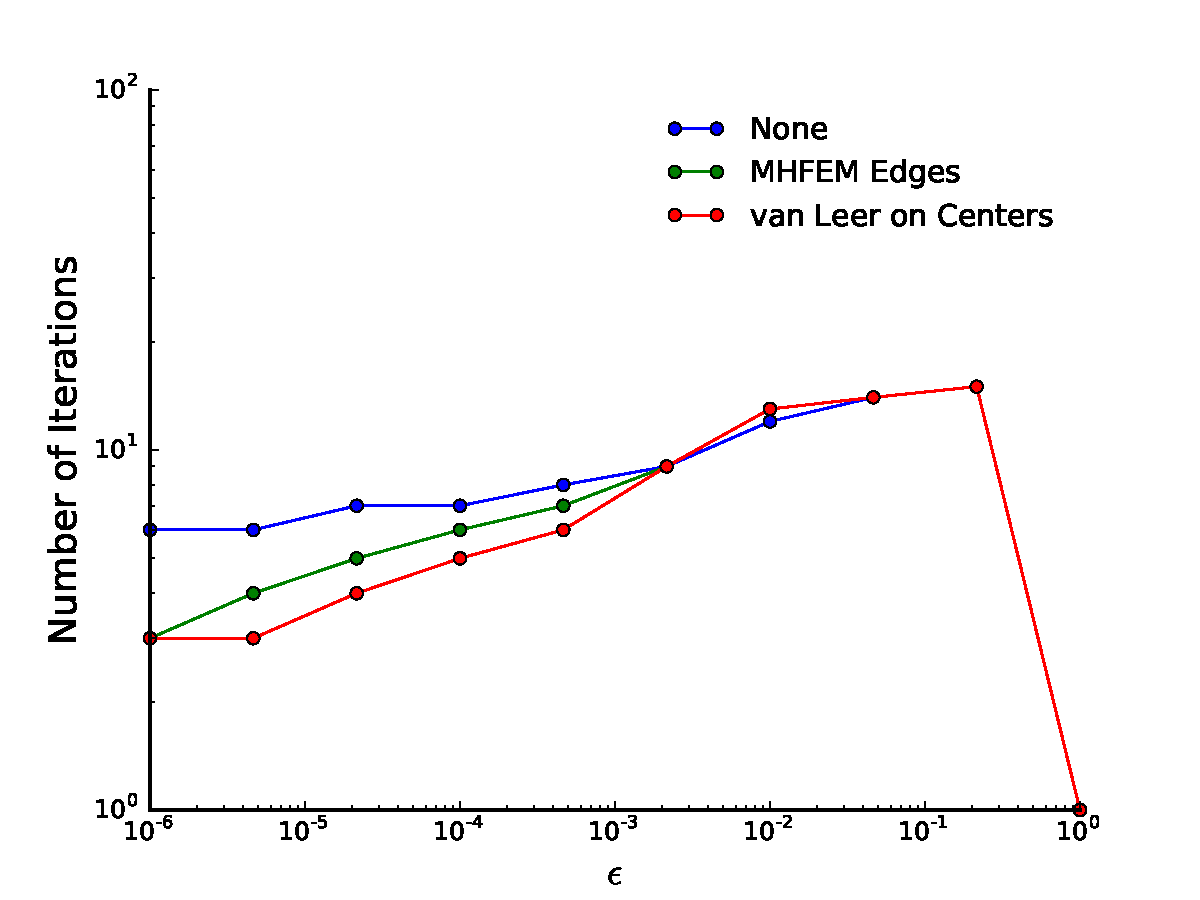
\includegraphics[width=.75\textwidth]{figs/diffLimit.pdf}
		\caption{The number of iterations for the VEF method to converge in the limit as $\epsilon \rightarrow 0$.}
		\label{fig:diffLim_iterations}
	\end{figure}
	\begin{figure} \centering
		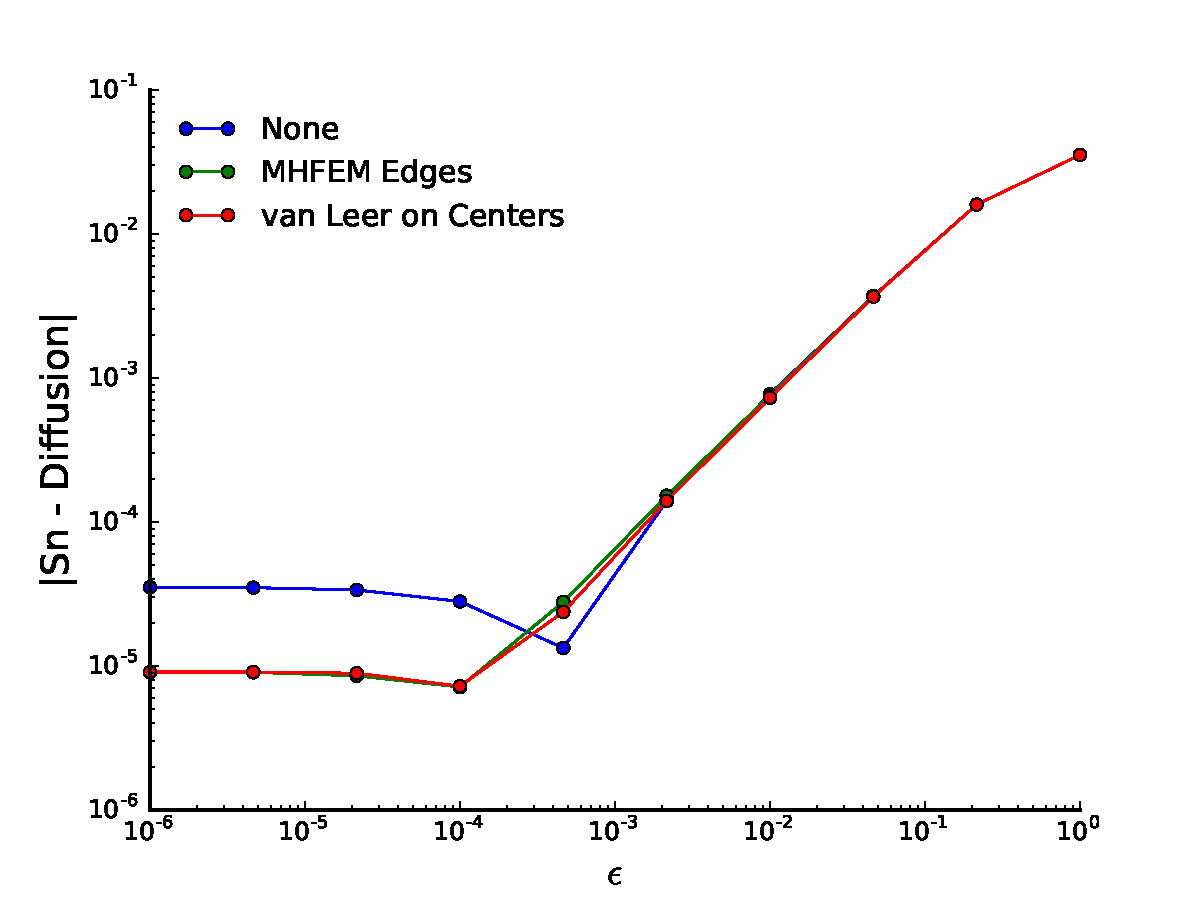
\includegraphics[width=.75\textwidth]{figs/diffError.pdf}
		\caption{A plot of the error between Diffusion Theory and the VEF solution as $\epsilon\rightarrow 0$. }
		\label{fig:diffLim_error}
	\end{figure}

\subsection{Solution Convergence}
The convergence between unaccelerated SI and the VEF method was compared as a function of cell width for a simple homogeneous slab and for a variant of Reed's problem. In both cases, the slab had a reflecting left boundary and vacuum right boundary. The homogeneous slab had a scattering ratio of 0.75. The cross sections and source for Reed's problem are provided in Table \ref{tab:reedXS}. Figure \ref{fig:reed} shows the L2 norm of the difference between unaccelerated and VEF accelerated S$_8$ for the two test problems. 

	\begin{table} \centering
		\begin{tabular}{|c|c|c|c|c|c|}
			\hline
			& Region 1 & Region 2 & Region 3 & Region 4 & Region 5 \\ 
			\hline 
			$q$ & 50 & 0 & 0 & 0 & 1 \\ 
			$\Sigma_t$ & 50 & 0.001 & 1 & 5 & 1 \\ 
			$\Sigma_a$ & 50 & 0 & 0.1 & 0 & 0.1 \\ 
			\hline 
			Domain & $0 \leq x < 2$ & $2 \leq x < 4$ & $4\leq x < 6$ &
				$6 \leq x < 7$ & $7 \leq x \leq 8$\\ 
			\hline 
		\end{tabular}
		\caption{The cross sections and source used for Reed's problem.}
		\label{tab:reedXS}
	\end{table}

	\begin{figure} \centering
		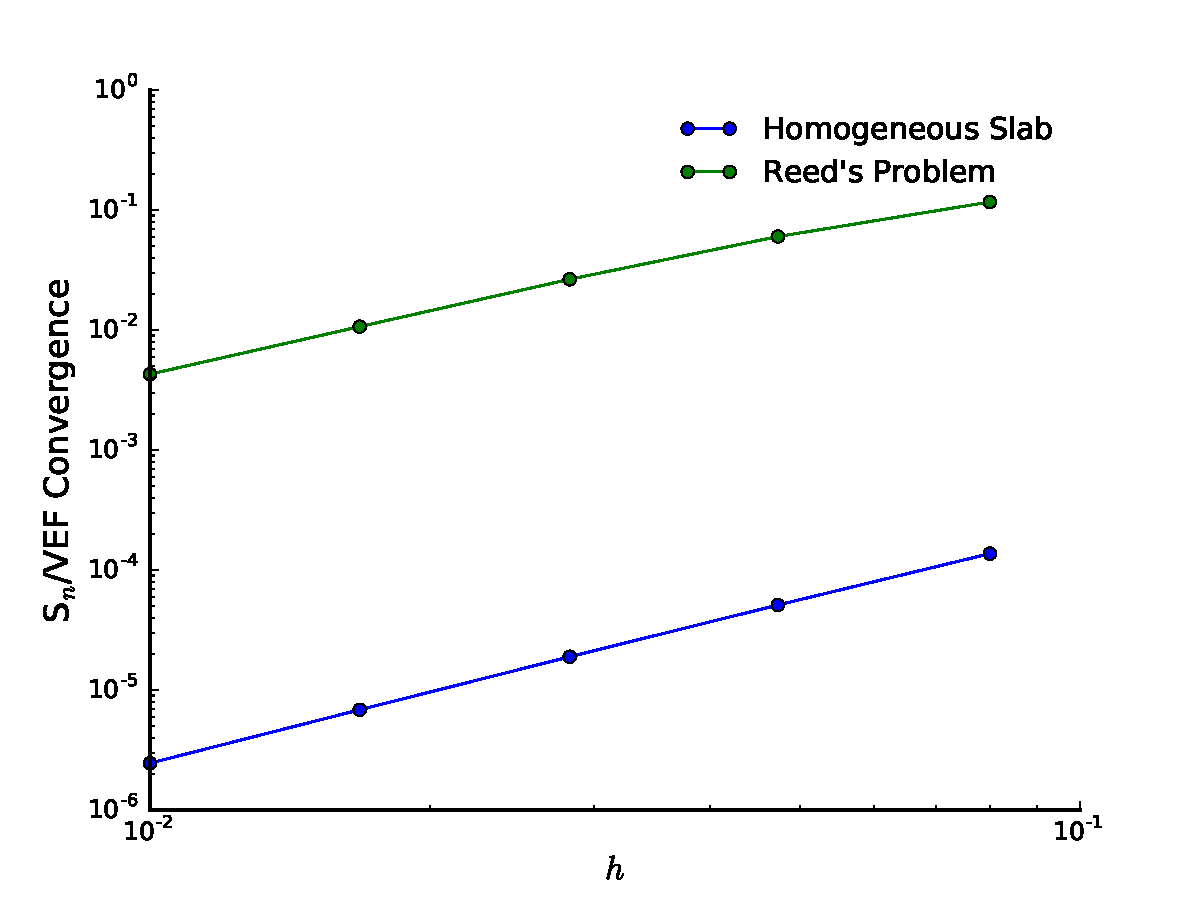
\includegraphics[width=.75\textwidth]{figs/convergence.pdf}
		\caption{The L2 norm of the difference between unaccelerated and VEF S$_8$ for a homogeneous slab and Reed's problem. }
		\label{fig:reed}
	\end{figure}

In both cases, the \SN and VEF solutions converge as the cell width is decreased. The convergence for Reed's problem is three orders of magnitudes worse than for the homogeneous slab case. This suggests that 

\subsection{Comparison to S$_2$SA}

